\documentclass[svgnames]{standalone}
\usepackage{tikz}
\usetikzlibrary{calc,positioning,backgrounds,arrows}

% Define constants here

\begin{document}
		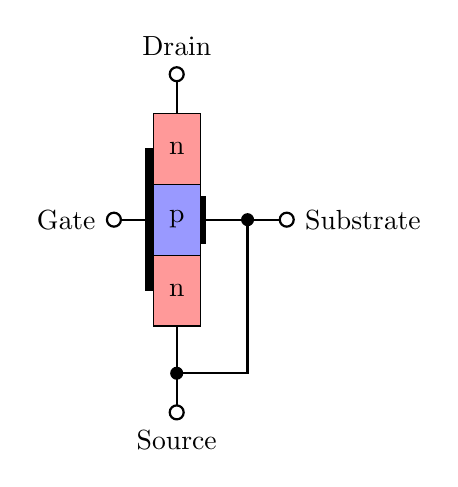
\begin{tikzpicture}[scale=0.3]
			\filldraw[fill=blue!40!white, draw=black] (0,0) rectangle ++(2,3) node[pos=.5] {p};
			\filldraw[fill=red!40!white, draw=black] (0,3) rectangle ++(2,3) node[pos=.5] {n};
			\filldraw[fill=red!40!white, draw=black] (0,0) rectangle ++(2,-3) node[pos=.5] {n};
			\draw [thick, -o] (0, 1.5) -- ++(-2,0) node[anchor=east] {Gate};
			\draw [thick, -o] (1, 6) -- ++(0,2) node[anchor=south] {Drain};
			\draw [thick, -o] (1, -3) -- ++(0,-4) node[-*, anchor=north] {Source};
			\draw [thick, -o] (2, 1.5) -- ++(4,0) node[-*, anchor=west] {Substrate};
			\draw [thick] (4, 1.5) node[fill, circle, scale=0.5] {} -- ++(0,-6.5) -- ++(-3, 0) node[fill, circle, scale=0.5] {};
			\filldraw [fill=black, draw=black] (0, -1.5) rectangle ++(-0.3,6);
			\filldraw [fill=black, draw=black] (2, 0.5) rectangle ++(0.2,2);
		\end{tikzpicture}
\end{document}
